% Diese Zeile bitte -nicht- aendern.
\documentclass[course=erap] {aspdoc}

%eigene Imports
\usepackage{amsfonts}
\usepackage{pgfplots}
\pgfplotsset{compat=1.16}

%%%%%%%%%%%%%%%%%%%%%%%%%%%%%%%%%
%% TODO: Ersetzen Sie in den folgenden Zeilen die entsprechenden -Texte-
%% mit den richtigen Werten.
\newcommand{\theGroup}{233} % Beispiel: 42
\newcommand{\theNumber}{A316} % Beispiel: A123
\author{Ludwig Gröber \and Julian Pins \and Daniel Safyan}
\date{Sommersemester 2023} % Beispiel: Wintersemester 2019/20
%%%%%%%%%%%%%%%%%%%%%%%%%%%%%%%%%

% Diese Zeile bitte -nicht- aendern.
\title{Gruppe \theGroup{} -- Abgabe zu Aufgabe \theNumber}

\begin{document}
    \maketitle


    \section{Einleitung}
    Die gegebene Aufgabenstellung A316 verlangt die Implementierung der Funktion f(x)=arsinh(x) im C17 Standard von C.
    Wie die angewandte Methodik und der mathematische Lösungsansatz aussieht, wird im Folgenden beschrieben.

    \subsection{Einführung 1/2Seite}
    %Allgemeine Einführung und Abwägung bei Optimierungen
    Im Folgenden wird ein Problem aus dem Bereich der optimierung von Programmen behandelt.
    Diese Optimierung kann unter verschiedenen im Folgenden erläuterten Kriterien erfolgen.
    Die Optimierung vom Programmen ist im Allgemeinen immer ein Abwägen zwischen Implementierungsaufwand/Laufzeit in Zyklen/Laufzeit in Zeit/Energieaufwand/Portabilität/Speicherverbrauch und weiteren Anwendungsspezifischen Faktoren.
    Diese Abwägungen werden im Folgenden auch bei unserer Implementierung getroffen und und es wir versucht ein 'optimales' Ergebnis in verschiedenen Dimensionen zu erzielen, zu messen und zu bewerten.
    Hierbei dient uns der Vergleich als Bewertungskriterium und die bewerteten Dimensionen werden in den weiteren Kapiteln noch genauer spezifiziert.
    Eine Bewertung der Ergebnisse erfolgt am Ende des Kapitels Performanzanalyse.


    %Motivation
    Die Gruppe der hyperbolischen Funktionen wird für die Hankel-Transformation~\cite{hankel} ,
    bei der Lösung bestimmter Differenzialgleichungen~\cite{differenzial}, bei der Beschreibung von Katenoiden~\cite{katenoid}
    sowie in den Friedmann-Gleichungen für die zeitliche Entwicklung der Ausdehnung des Universums~\cite{universum1,universum2}~ benötigt.
    Für diese üblicherweise rechenintensiven Anwendungen ist eine effiziente und genaue Implementierung aller dafür verwendeten Funktionen essenziell um Gesamtergebnisse effizient erzielen zu können.
    Deshalb widmed sich diese Ausarbeitung im folgenden der Implementierung einer hyperbolischen Funktion, dem $arsinh$.

    \subsection{Aufgabenstellung analysiert und spezifiziert 1/2Seite}
    Die gestellte Aufgabe verlangt die numerische Berechnung der Funktion f(x) = arsinh(x) im C17 Standard von C.


    %Mathematische Analyse
    Über den komplexen Zahlen $\mathbb{C}$ bildet die Funktion $arsinh$ mehrwertig ab, weshalb die Einschränkung auf die reellen Zahlen $\mathbb{R}$ getroffen wird.
    Die Funktion area sinus hyperbolicus bildet über $\mathbb{R}$ nach $\mathbb{R}$ ab und ist im Bereich $-\infty < x < + \infty$ definiert.
    Der area sinus hyperbolicus kann über den Logarithmus, über ein Integral oder über den $sinh$ definiert werden.

    $$ (1) \operatorname{arsinh}(x) = \ln \left(x + \sqrt{x^2 + 1} \right) \, mit \, x \in \mathbb{R}$$

    $$ (2) \operatorname{arsinh}(x) = \int\_{0}^{1} \frac{x}{\sqrt{x^2 y^2 + 1}} \,\mathrm{d}y \, mit \, x \in \mathbb{R} $$

    $$ (3) \operatorname{arsinh}(x) = \frac{1}{sinh(x)} $$

    Im Limit kann er durch die Funktion $f(x)\to \pm \ln(2|x|)$ angenähert werden.
    Als für die Implementierung relevante mathematische Eigenschaft die Punktsymmetrie zum Ursprung $(0,0)$ bereits hier zu erwähnen.


    Die Familie der hyperbolischen Funktionen sind quadratische rationale Funktionen von der Exponentialfunktion $\exp$,
    die über die Mitternachtsformel gelöst werden könnten und mit dem natürlichen Logarithmus $\ln$ ausgedrückt werden.


    %Überleitung
    Bei der Abbildung einer stetigen Funktion in ein endliches System müssen zudem Einschränkungen im Wertebereich sowie bei der Genauigkeit getroffen werden.


    %Implementierung
    Letzteres wird im eigens dafür angelegten Kapitel "Genauigkeit" diskutiert, allgemein kann jedoch bereits zum Datentyp $double$ erwähnt werden, dass bei 52 Fragment-bits eine dezimale Genauigkeit von $53*\log10(2) \approx 15,96$ die Grenze des Datentyps darstellt.~\cite{StandardforBinaryFloating-PointArithmetic}
    Erstere Grenze gibt die Aufgabenstellung indirekt durch die doppelte Genauigkeit der Fließkommaarithmetik vor.
    Der Wertebereich der Implementierung ist ebenso durch den Datentypen $double$ beschränkt $\min(double) =  = 2,2250738585072014* 10^308$ und $\max(double) =  = 1,7976931348623157 * 10^308$


    Die Werte $\pm \infty$ und $\pm NaN$ sind bei $double$ besonders zu beachten.
    Da die Funktion streng monoton steigend ist, definieren wir:
    \[(4) \operatorname{arsinh}(x) =
    \begin{cases}
        arsinh(x)     & \text{ falls } x < \infty \wedge \, x > -\infty \\
        +NaN  & \text{ falls } x = +NaN \\
        -NaN  & \text{ falls } x = -NaN \\
        +\infty     & \text{ falls } x = +\inf \\
        -\infty     & \text{ falls } x = -\inf \\
        +NaN     & \text{ sonst }

    \end{cases}\]


    Ein Problem bei $double$ ist zudem die Endianness, die nicht in IEEE 754~\cite{StandardforBinaryFloating-PointArithmetic} spezifiziert ist.
    Es könnte also zu Fehlern zwischen Systemen kommen, die Behandlung dessen übersteigt den Umfang diese Ausarbeitung und wird deshalb aus dem Themenbereich ausgeschlossen.


    Neben den sich aus dem Datentyp ergebenden Einschränkungen stellt die Aufgabenstellung ebenso Einschränkungen an arithmetischen Operatoren.
    In der ersten naiven Ausarbeitung dürfen nur grundlegende Berechnungen, also die vier Grundrechenarten sowie shifts verwendet werden.
    In der weiterführenden Ausarbeitung sind komplexe Berechnungen wie $exp$ oder $log$ sowie SIMD, SSE zugelassen und weitere Optimierungen wie Loop-unrolling, Endrekursion, die Wahl anderer Algorithmen und Datenstrukturen erlaubt und erwünscht.


    Von den beiden geforderten Vergleichsimplementierungen als Reihenentwicklung und als Tabellen-Lookup ist letztere bereits als eine Form der Optimierung zu verstehen.
    Und kann deshalb bereits mit der Reihe, ceteris paribus, verglichen werden.
    Tabellen-Lookup scheint für die gegebene Aufgabe eine gute Optimierung zu sein, da für eine bekannte Menge an Funktionswerten häufige und identische Berechnungen durchgeführt werden.
    Die Wahl der größe eines Tabellen-Lookups ist eine Abwägung zwischen Laufzeit und Speicherplatz, dies wird im Folgendem Kapitel "Optimierungen" weiter erläutert.


    Gemäß Aufgabenstellung sollen also drei C-Implementierungen erarbeitet und verglichen werden.


    (A) Eine Implementierung als reine Reihendarstellung mit grundlegenden Berechnungen


    (B) Eine Implementierung als Tabellen-Lookup mit grundlegenden Berechnungen


    (C) Hauptimplementierung: Eine Implementierung nach freier Wahl mit komplexen Instruktionen


    Im folgenden werden die Implementierungen mit den Buchstaben $(A)$, $(B)$ und $(C)$ referenziert, die Formeln analog mit den Zahlen.
    $A$ wird im Folgenden als naive Implementierung und als Benchmark für die Performanz verwendet.


    Das Rahmenprogramm unterstützt die Funktionen $-V<Zahl>$ für die Wahl der Implementierung, $-B<Zahl>$ für die Wiederholungen des Funktionsaufrufs, $<Floating Point Zahl>$ für den Wert $x$, $-h$ oder $--help$ für die Beschreibung der Optionen des Programms und Verwendungsbeispiele hierfür.


    Eine Implementierung in Assembly ist nicht gefordert und es wird in dieser Ausarbeitung auch darauf verzichtet, da der Fokus im Folgenden auf Genauigkeit und nicht auf Performanz liegen wird.
    Ebenso verzichten wir auf Mikro-Optimierungen, da es allgemein schwer ist moderne Compiler in Optimierungsaufgaben zu schlagen und der Code hierdurch schwerer zu lesen, fehleranfälliger und schwerer zu warten wird.
    Dies steht allgemein best-practices im Software-Engineering entgegen.

    %% TODO: benötigt?
    Intervalle werden größer an den Rändern, weil double precision nicht so genau ist.
    Relativer Fehler bleibt gleich an jeder Stelle.


    \section{Lösungsansatz}

    % Theoretischer Teil
    In diesem Absatz rechtfertigen wir die beiden Ansätze der Reihenentwicklung und des Tabellen-Lookups mathematisch.
    Sowohl die Polynominterpolation als auch die intervallweise lineare Interpolation sind 

    \subsection{Reihendarstellung}
    Die 





    Leiten Sie mathematisch zwei Möglichkeiten her, die Funktion zu berechnen.
    Verwenden Sie dazu sowohl eine reine Reihendarstellung als auch eine Methodik, die einen Tabellen-Lookup benutzt.

    Ideen: Reihenentwicklung nicht zur Runtime, sondern zur Compiletime berechnen.
    Runge Effekt: zwischen Integralgrenzen gut angenähert, wenn mit Polynom genähert wird. -> Deshalb funktioniert die Reihenentwicklung nicht.
    Lösung: Splines über großen Bereich mit x^3 Polynom annähern. Intervall gleich verteilt. alpha x^3 + beta x^2 + gamma x + delta
    Annäherung für große Werte: x^2 + 1 = x^2
    Ableitung per Tailor-Reihe
    Idee: 1. Chilliger Lookup Table mit Interpolation 2. Splines Lookup Table
    Entwicklung als echte Reihendarstellung muss begrenzt werden im Wertebereich.

    Grunstätzlich möglichst wenig zur Runtime berechnen.
    Reihe: Basisfunktionen + Lineares Gleichungssystem
    Lagrange Polynome
    Tailor-Reihe / Tailor Entweicklung

    \subsection{Naive Implementierung Reihenentwicklung ]-1/1[}

    \subsection{Naive Implementierung Tabellen-Lookup ]-Inf/+Inf[}

    \subsection{Vergleich der beiden Ansätze}

    \subsection{Optimierte Implementierung Reihenentwicklung ]-1/1[}
    Complexe Instruktionen, Wurzel, Log, Exponent, SIMD?

    \subsection{Optimierte Implementierung Tabellen-Lookup ]-Inf/+Inf[}
    Idee: Hash-Map

    \subsection{Implementierung mit komplexen Instruktionen}


    \section{Genauigkeit}
    Im gegebenen Kontext ist die Genauigkeit der Lösung als die Abweichung der Implementierung $(4)$ vom Funktionswert der mathematisch definierten Funktion $(1)$ zu verstehen.


    \section{Performanzanalyse}
    Die Performanz der Implementierungen wird anhand der Laufzeit gemessen.
    Die Laufzeit ist mit der Libaray $time.h$ gemessen worden.
    Hierbei sind einige Dinge vorab zu definieren: 

    
    %Voraussetzungen
    Getestet wurde auf einem System mit Intel i5-10210U Prozessor, 1.60 GHz, 8 GiB Arbeitsspeicher, Ubuntu 22.04.2 LTS, 64 Bit, 5.19.0-46-generic Linux-Kernel. Kompiliert wurde mit GCC 11.3.0 mit der Option -O3. Da die Laufzeit aller drei Implementierungen nur minimal von der Größe der Eingabewerte abhängt, haben wir uns dafür entschieden, die Laufzeitmessung mit einigen repräsentativen Werten verschiedener Größenordnungen durchzuführen. Es wurden mit 10 verschiedenen Werten jeweils 100.000.000 mal die Funktionen aufgerufen, um dann die durchschnittliche Zeit für einen Funktionsaufruf zu ermitteln. Der folgende Graph zeigt die durchschnittliche Laufzeit der drei Implementierungen mit Reihenentwicklung, Tabellenlookup und komplexen Instruktionen der C-library in Nanosekunden.

    %Tabelle
    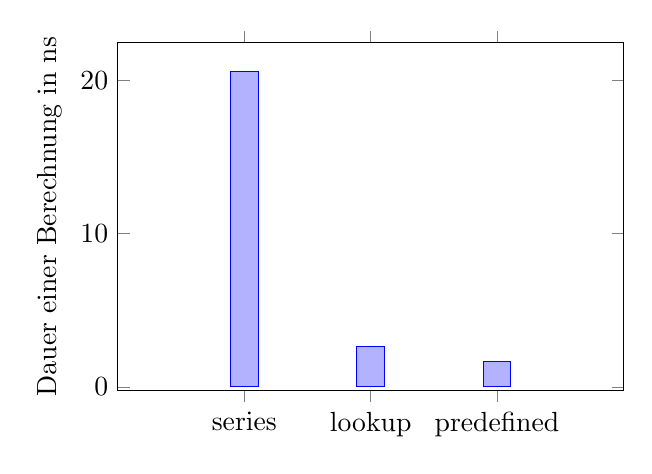
\begin{tikzpicture}
    \begin{axis}[
    ybar, 
    width= 8cm, height = 6 cm,
    enlarge x limits = 0.5, 
    ylabel = {Dauer einer Berechnung in ns},
    symbolic x coords = {series, lookup, predefined},
    xtick=data,
    ]
    \addplot coordinates
    {(series, 20.565) (lookup, 2.613) (predefined, 1.648)};
    \end{axis}
    \end{tikzpicture} 

    %Folgerungen
    Wie in Abb.7 zu sehen ist, ist die reine Reihen-Implementierung um ein Vielfaches(bis zu 12x) langsamer als die anderen
    beiden Vergleichsimplementierungen. Hier liegt wirklich die Stärke einer Implementierung durch Lookuptable, da wir hier für jeden
    Input nur sehr billige arithmetische Ausdrücke zum linearen Interpolieren verwenden. Die Reihenentwicklung andererseits verwendet 
    viele Multiplikationen und Divisionen über mehrere Iterationen, was jedoch als Reihendarstellung mit Polynomen von uns erwartet
    wurde. Die Implementierung mit komplexen Instruktionen ist noch etwas schneller als unser Lookuptable, ist jedoch als Teil der 
    C-library schwer zu unterbieten. Bei unseren einem unserer 3 grundlegenden Ziele: Genauigkeit wird die Reihenentwicklung folglich von demä
    Lookup-Table stark outperformt. 

    \subsection{Methodik und Annahmen 0,5Seite}
    Um optimale Vergleichbarkeit der Ergebnisse sicher zu stellen, versuchen wir eine möglichst exklusive nutzung der Maschine sicher zu stellen.
    Hierfür wurden alle nicht für das jeweilige Betriebssystem nötigen Prozesse beendet, alle Programme geschlossen, die Maschine an das Stromnetz angeschlossen und die Kühlung manuell auf die höchste Stufe gesetzt.
    Dies soll Performanceänderungen aufgrund von Überhitzung bei mehrfacher Ausführung vermeiden.
    Um einen stabilen Mittelwert zu erzielen, wird jede Implementierung mindestens 10 mal ausgeführt, nähere Angaben dazu sind der jeweiligen Messung zu entnehmen.

    Alle Performaztests werden auf folgender Maschine ausgeführt: Name: ____ Prozessor: ____ Takt: ____ Multicore/SingleCore Speicher: ____ Betriebssystem: _____ Compiler: ____ Version: ____ Comilerflags: siehe Makefile

    Die Tests werden mit den Eingaben ____ ausgeführt und ____ mal wiederholt.

    Da es sich in der Aufgabe um eine numerische Berechnung handelt, erwarten wir bei den Performanztests lediglich Algorithmisch bedingte Abweichungen, welche durch die Laufzeitklassen beschrieben werden könnten.
    Implementierung $A$: $O(7)$
    Implementierung $B$: $O(1)$
    Implementierung $C$: $O(1)$

    \subsubsection{Zeitmesung der naiven Reihenentwicklung}

    \subsubsection{Zeitmesung des naiven Tabellen-Lookup}

    \subsubsection{Zeitmesung des optimierten Tabellen-Lookup}
    ziehen Sie als weiteren Vergleich eine C-Implementierung unter Nutzung von komplexeren Instruktionen, die beispielsweise eine Wurzelberechnung durchführen, heran.

    \subsection{Bewertung, Einordnung und Erklärung der Ergebnisse}


    \section{Zusammenfassung und Ausblick}

    Zusammenfassend lässt sich feststellen, dass der Trade-off zwischen Performance, Genauigkeit und Speicherverbrauch für die beiden Implementierungen mit einem Tabellenlookup beziehungsweise einer Reihenentwicklung sehr unterschiedlich ist. Der Tabellenlookup ist zwar sehr schnell, benötigt allerdings auch immer mehr Speicherplatz, je genauere Werte man erhalten möchte. In unserer Implementierung, die insgesamt ca. 30000 Werte in einer Lookuptabelle speichert, hat die Berechnung einen maximalen relativen Fehler von bis zu etwa 0.01 Prozent. 
    
    Die Reihenentwicklung auf der anderen Seite liefert zumindest für x-Werte, deren Betrag nicht nahe an Eins liegt, bereits mit wenigen Reihengliedern deutlich exaktere Werte. Allerdings werden beide Reihen für eine konstante Anzahl an Reihengliedern immer ungenauer, je näher sich x Eins annähert - um das exakte Ergebnis für Eins zu erhalten wäre eine unvertretbar hohe Anzahl an Reihengliedern erforderlich, die zu extremen Performanzeinbußen führen würden.
    Auch für die 20 Reihenglieder, für die wir uns entschieden haben, benötigt die Reihenentwicklung bis zu 12 mal so lange für die Berechnung, dafür benötigt sie auch deutlich weniger Speicherplatz. 

    Welches Programm verwendet werden sollte, hängt also stark von den Rahmenbedingungen ab. 
    In der Statistik kann der Areasinus Hyperbolicus zur Modellierung von Verteilungen verwendet werden, während er im Bereich des Ingenierwesens Anwendung in der Modellierung und Analyse von Systemen, beispielsweise in Steuerungs- und Regelungstechnik findet. Für die Auswertung großer Messreihen zu diesem Zweck eignet sich die Lookuptabelle deutlich besser, da Messungen in der Regel sowieso einen kleinen Fehler aufweisen und die Lookuptabelle für viele Werte aufgrund der besseren Performanz schneller Ergebnisse liefert. 
    Hat jedoch die exakte Genauigkeit der Ergebnisse ein höhere Priorität, so eignet sich die Reihenentwicklung mehr. Für x-Werte nahe an Eins müssen allerdings sehr viele Reihenglieder berechnet werden, da das Ergebnis andernfalls dennoch ungenau ausfällt. 

    \subsection{Ausblick}

    In unserer Implementierung des Areasinus Hyperbolicus haben wir uns auf eine reine Reihenentwicklung und eine recht simple Lookuptabelle mit linearer Näherung beschränkt. Unter weniger strengen Rahmenbedingungen ließe sich die Implementierung allerdings sowohl in Bezug auf Laufzeit, als auch Genauigkeit noch signifikant optimieren. 
    Ein möglicher Ansatz ist die Verwendung von Splines in der Lookuptabelle: Statt der bisher linearen Näherung zwischen zwei Messpunkten in der Lookuptabelle, könnte man den areasinus hyperbolicus in diesem Intervall durch eine Kurven annähern. Hierzu werden in der Regel Polynome vom Grad drei verwendet. Dadurch verbessert sich die Genauigkeit, insbesondere für x-Werte die genau zwischen zwei Werten in der Lookutabelle liegen deutlich, während sich die Laufzeit nur minimal erhöht. Dafür steigt allerdings der benötigte Speicherplatz, da nun für jedes Intervall ein Polynom gespeichert werden muss.
    
    Ein weiterer Ansatz wäre, eine Kombination aus Reihenentwicklung und Lookuptabelle zu verwenden: 

    Die Wahl des Datentyp $double$ bietet eine einfache Möglichkeit zur Erhöhung der Genauigkeit oder zur Verkleinerung des Speicherverbrauchs.
    Gemäß IEEE 754 ~\cite{StandardforBinaryFloating} könnte auch die einfache oder vierfache Genauigkeit der
    Fließkommaarithmetik gewählt werden, wodurch sich die Genauigkeit auf $23*\log10(2) \approx 6,92$ dezimale Nachkommastellen
    bzw. $112*\log10(2) \approx 33,72$ dezimale Nachkommastellen respektive verändern würde.
    Der Speicherverbrauch würde sich bei einfacher Genauigkeit von 64 bit auf 32 bit halbieren, bei vierfacher Genauigkeit von 64bit auf 128bit verdoppeln.
    Hierbei ist je nach Anwendung die entsprechende Abwägung zu treffen.


% TODO: Fuegen Sie Ihre Quellen der Datei Ausarbeitung.bib hinzu
% Referenzieren Sie diese dann mit \cite{}.
% Beispiel: CR2 ist ein Register der x86-Architektur~\cite{intel2017man}.
    \bibliographystyle{plain}
    \bibliography{Ausarbeitung}
% Sämtliche in der Ausarbeitung verwendeten Quellen sind hier aufzuführen.
% Es sollen nur zitierfähige Quellen verwendet werden. Wir empfehlen die Verwendung von BibTEX.

\end{document}